\documentclass[a4paper,12pt]{article}
\usepackage{amssymb}
\usepackage{amsmath}
\usepackage[utf8]{inputenc} % Umlaute
\usepackage[ngerman]{babel} % Umlaute
\usepackage[T1]{fontenc}    % Umlaute
\usepackage[margin=2.5cm]{geometry}
\usepackage{booktabs}
\usepackage{lmodern}

% Notwendig für Links im Text
\usepackage{hyperref}

% glossar, see http://en.wikibooks.org/wiki/LaTeX/Glossary
% muss NACH hyperref geladen werden, sonst funktionieren die Links nicht
\usepackage{glossaries}

% Kompatibilität
\ifx\pdftexversion\undefined
\usepackage[dvips]{graphicx}
\else
\usepackage[pdftex]{graphicx}
\DeclareGraphicsRule{*}{mps}{*}{}
\fi

\makeglossaries

%%%%%%%%%%%%%%%%%%%%%%%%%%%%%%%%%%%%%%%%%%%%%%%%%%%%%%%%%%%%%%%%%%%%%%
% Variablen                                 						 %
%%%%%%%%%%%%%%%%%%%%%%%%%%%%%%%%%%%%%%%%%%%%%%%%%%%%%%%%%%%%%%%%%%%%%%
\newcommand{\authorName}{Test, Test, Test, Test, Test, Test, test}
\newcommand{\auftraggeber}{Karlsruhe Institute of Technology (Teco)}
\newcommand{\auftragnehmer}{wir}
\newcommand{\projektName}{Earables}
\newcommand{\tags}{\authorName, Pflichtenheft, KIT, Informatik, PSE}
\newcommand{\glossarName}{Glossar}
\title{\projektName~(Pflichtenheft)}
\author{\authorName}
\date{\today}

%%%%%%%%%%%%%%%%%%%%%%%%%%%%%%%%%%%%%%%%%%%%%%%%%%%%%%%%%%%%%%%%%%%%%%
% PDF Meta information                                 				 %
%%%%%%%%%%%%%%%%%%%%%%%%%%%%%%%%%%%%%%%%%%%%%%%%%%%%%%%%%%%%%%%%%%%%%%
\hypersetup{
  pdfauthor   = {\authorName},
  pdfkeywords = {\tags},
  pdftitle    = {\projektName~(Pflichtenheft)}
}

%%%%%%%%%%%%%%%%%%%%%%%%%%%%%%%%%%%%%%%%%%%%%%%%%%%%%%%%%%%%%%%%%%%%%%
% Create a shorter version for tables. DO NOT CHANGE               	 %
%%%%%%%%%%%%%%%%%%%%%%%%%%%%%%%%%%%%%%%%%%%%%%%%%%%%%%%%%%%%%%%%%%%%%%
\newcommand\addrow[2]{#1 &#2\\ }

\newcommand\addheading[2]{#1 &#2\\ \hline}
\newcommand\tabularhead{\begin{tabular}{lp{13cm}}
\hline
}

\newcommand\addmulrow[2]{ \begin{minipage}[t][][t]{2.5cm}#1\end{minipage}%
   &\begin{minipage}[t][][t]{8cm}
    \begin{enumerate} #2   \end{enumerate}
    \end{minipage}\\ }

\newenvironment{usecase}{\tabularhead}
{\hline\end{tabular}}

\usepackage{microtype}
%%%%%%%%%%%%%%%%%%%%%%%%%%%%%%%%%%%%%%%%%%%%%%%%%%%%%%%%%%%%%%%%%%%%%%
% GLOSSARY ENTRIES                 	                              	 %
%%%%%%%%%%%%%%%%%%%%%%%%%%%%%%%%%%%%%%%%%%%%%%%%%%%%%%%%%%%%%%%%%%%%%%

\newglossaryentry{Echtzeit}{name=Echtzeit, description={Bereitstellen/Anzeigen von Daten mit einer durch die Verarbeitung bedingten Verzögerung von bis zu ca. 2 Sekunden zwischen dem Anfallen der (Roh-)Daten und der Ausgabe bzw. Visualisierung.}}
\newglossaryentry{Vorgang}{name=Vorgang, description={Als Vorgang wird in diesem Pflichtenheft bezeichnet, wenn ein Modus ausgewählt ist und Start gedrückt wurde. Der Vorgang endet mit dem Drücken von Stopp bzw. wird mit dem Wechseln des Modus.}} %%brauchen wir noch ne abbrechen Taste in der gui? haben wir so was schon?
\newglossaryentry{BLE}{name=BLE, description={Bluetooth Low Energy ist eine Technologie, die Teil des Industriestandards Bluetooth ist und eine energiesparende, kabellose Kommunikation zwischen Geräten in einer Entfernung von bis zu ca. 10 Metern ermöglicht.}}
\newglossaryentry{Wearable Computings}{name=Wearable Computings, description={Unterdem Begriff Wearable Computings versthet man, Computerysyteme die am Körper, unter der Kleidung oder als Implantat unter der Haut getragen werden können.}}
\newglossaryentry{6-Achsen IMU}{name=6-Achsen IMU, description={Ein 6-Achsen IMU ist ein Beschleunigungssensor mit Gyroskop.}}
\newglossaryentry{GUI}{name=GUI, description={GUI ist die Abkürzung für den englischen Begriff "graphical user interface". Sie ist die Schnittstelle zwischen Mensch und Maschine und ermöglicht dem Nutzer die Eingabe/Steuerung, der Maschine.}}
\newglossaryentry{Cross-Platform Bibliothek}{name=Cross-Platform Bibliothek, description={Eine Cross-Platform Bibliothek ist nichts weiter als eine Bibliothek die auf Rechnersystemen mit verschiedener Architektur laufen kann.}}
\newglossaryentry{Steuerungsparameter}{name=Steuerungsparameter, description={Steuerungsparameter sind Parameter, mit denen ein Programm eingestellt werden kann, um auf eine bestimmte Art und weiße zu arbeiten.}}
\newglossaryentry{Schrittfrequenz}{name=Schrittfrequenz, description={Die Schrittfrequenz gibt an wie viele Schritte pro Zeiteinheit gemacht werden.}}
\newglossaryentry{Rohdaten}{name=Rohdaten, description={Als Rohdaten werden unverarbeitete Daten bezeichnet.}}
\newglossaryentry{TTS}{name=Text-To-Speech, description={Ein Text-to-Speech-System (TTS) (oder Vorleseautomat) wandelt Fließtext in eine akustische Sprachausgabe um.}}
\newglossaryentry{Earables}{name=Earables, description={Eine Amalgamierung des Wortes Wearable und Earphone. Dabei handelt es sich um Kopfhörer, die mit Sensoren ausgestattet sind.}}


%%%%%%%%%%%%%%%%%%%%%%%%%%%%%%%%%%%%%%%%%%%%%%%%%%%%%%%%%%%%%%%%%%%%%%
% THE DOCUMENT BEGINS             	                              	 %
%%%%%%%%%%%%%%%%%%%%%%%%%%%%%%%%%%%%%%%%%%%%%%%%%%%%%%%%%%%%%%%%%%%%%%
\begin{document}
 \pagenumbering{roman}
 \begin{titlepage}
\maketitle
\thispagestyle{empty} % no page number

\begin{verbatim}












\end{verbatim}


  \begin{tabular}[t]{p{4 cm}p{8 cm}}
	Projekt:       & \projektName \\[1.2ex]
	Auftraggeber:  & \auftraggeber\\[1.2ex]
	Auftragnehmer: & \auftragnehmer\\[1.2ex]
  \end{tabular}


\begin{tabular}[t]{|p{4 cm}|p{8 cm}|}
\hline
\textbf{Datum} & \textbf{Autor(en)} \\
\hline
\hline
\today & \authorName \\
\hline
\end{tabular}
\end{titlepage}
         % Deckblatt.tex laden und einfügen
 \setcounter{page}{2}
 \tableofcontents          % Inhaltsverzeichnis ausgeben
 \clearpage
 \pagenumbering{arabic}

\section{Einleitung}
%% BLE glossareintrag konflikt
%%Wearable Computing ist laut wikipedia das Forschungsgebiet der Wearables/Wearable Computer...
%%Atemfrequenz durch Schrittfrequenz ersetzt
\Gls{Earables} gehören zu den \Gls{Wearable Computings}, sie sind also nichts anderes als intelligente Kopfhörer. Je nachdem wie sie ausgestattet werden bringen sie die unterschiedlichsten Funktionen mit sich. Neben der klassischen Ausstattung von Lautsprechern, Mikrophon und Bluetooth Low Energy besitzen sie in unserem Fall zusätzlich eine \Gls{6-Achsen IMU}. Mit ihrer Hilfe ist man in der Lage die Bewegungen des Nutzers zu erkennen und aufzuzeichnen, um mit den gewonnenen Messdaten  beispielsweise die Schrittfrequenz zu messen.  \Gls{Earables} bilden also eine Schnittstelle zwischen Mensch und Computer. Da sie kaum von normalen Bluetooth Kopfhörern zu unterscheiden sind, haben sie bereits jetzt eine hohe soziale Akzeptanz in der Gesellschaft erlangt, im Gegensatz zu beispielsweise Smartglasses. Mit der Entwicklung und Forschung dieser Art von \Gls{Earables} beschäftigt sich das globale eSense Projekt von Nokia Bell Labs in Zusammenarbeit mit dem Telecooperation Office (TECO). Hier wird gemeinsam nach möglichen Anwendungsfällen der \Gls{Earables} gesucht, wodurch auch dieses Projekt seinen Weg in diese Welt gefunden hat. %%Initiiert?
\section{Zielbestimmung}
Die Ziele dieses Projektes lassen sich in drei Bereiche gliedern:
\begin{enumerate}

  \item Es soll eine \Gls{Cross-Platform Bibliothek} (Android/IOS) für die \Gls{Earables} der Plattform eSense entwickelt werden mit der es möglich ist, die Messdaten des Gerätes aufzuzeichnen und verschiedene \Gls{Steuerungsparameter} zu verändern.
  
  \item Es soll ein Erweiterungsmodul entwickelt werden, mit dem die übermittelten  \Gls{Rohdaten} automatisch verarbeitet und ausgewertet werden, um so festzustellen ob der Nutzer gerade läuft oder steht.
  
  \item Es soll eine App mit einer \Gls{GUI} entwickelt werden, die über verschiedene Modi verfügt, insbesondere über einen der anzeigt, ob der Nutzer gerade läuft oder steht. 

\end{enumerate}

\subsection{Musskriterien}

  \begin{itemize}
    \item\text Die Cross-Platform Bibliothek soll in der Lage sein die gesammelten Daten der \Gls{Earables} aufzuzeichnen
    \item\text Die GUI der App muss so benutzerfreundlich gestaltet werden, dass der Benutzer intuitiv weiß wie man die Steuerungsparameter der \Gls{Earables} verändert
    \item\text Die Cross-Plattform Bibliothek soll in der Lage sein die verschiedenen Steuerungsparameter zu verändern.
    \item\text Das Erweiterungsmodul soll erkennen ob der Nutzer gerade \glqq läuft\grqq{}oder \glqq steht\grqq.
    \item\text Die App soll anzeigen können ob der Nutzer gerade läuft oder steht.
  \end{itemize}
\subsection{Wunschkriterien}
  \begin{itemize}
    \item\text Die App soll die \Gls{Schrittfrequenz} des Nutzers anzeigen.
    \item\text Die App soll die Anzahl der zurückgelegten Schritte anzeigen. %%Täglich? Gesamt?
    \item\text Die App soll die zurückgelegte Distanz anzeigen. %%Täglich? Gesamt?
    \item\text Die App soll über drei weitere Modi verfügen.
      \begin{itemize}
        \item\text Im Modus \glqq Zählmodus\grqq{} zählt die App wie viele Liegestützen oder Sit-ups der Nutzer macht.
        \item\text  Im Modus \glqq Lauschen\&Agieren\grqq{}kann der Nutzer seinen eigenen Trainingsplan erstellen, welcher dann über Text to Speech ausgegeben wird.
        \item\text  Im Modus \glqq Musikmodus\grqq{}wird die Musik automatisch gestoppt, wenn der Nutzer steht und wieder gestartet, wenn der Nutzer weiterläuft.
      \end{itemize}
    \item\text Die App wird standardmäßig auf Deutsch sein, der Nutzer soll weitere Sprachen durch Sprachpaket-Plugins hinzufügen können.
    \item\text Trainingsdaten werden automatisch gespeichert, Importieren und Exportieren soll möglich sein. %%Besprechen!
  \end{itemize}
  \subsection{Abgrenzungskriterien}
  \begin{itemize}
    \item\text Es werden keine Rohdaten längerfristig gespeichert. %%längerfristig ergänzt
    \item\text Die Musik passt sich nicht der Schrittfrequenz des Nutzers an.
    \item\text Im Modus \glqq Zählen\grqq{}wird davon ausgegangen, dass der Nutzer wirklich nur Liegestützen oder Sit-ups macht. Das bewusste Austricksen des Systems durch andere Bewegungen wird nicht behandelt.
    \item\text Es werden nur Daten auf dem Smartphone gespeichert und nicht auf den \Gls{Earables}
  \end{itemize}

\section{Produkteinsatz}
  \subsection{Zielgruppe}
  \begin{itemize}
    \item\textsf{Bibliothek:} Softwareentwickler
    \item\textsf{Erweiterungsmodul:} Softwareentwickler
    \item\textsf{App:} Hobbysportler
  \end{itemize}
  \subsection{Anwendungsbereiche}
    \begin{itemize}
      \item\textsf{Bibliothek} Softwareentwicklung für eSense Wearables
      \item\textsf{Erweiterungsmodul} Softwareentwicklung im Bereich Schritterkennung %%Vorschlag: Nutzung von Sensordaten als Nutzereingabe in einer App, z.b. im Fitness, aber auch für andere interaktive Apps ? (valle)
      \item\textsf{App} Heimtraining, Sport,\dots
    \end{itemize}
  \subsection{Betriebsbedingungen} %%macht nur für app sinn oder?
  %%TODO
  %mögliche Punkte: physikalische Umgebung (Training alleine, Umgebung egal), Betriebsdauer ("Akkuabhängig", keine weitere Grenzen), Qualifikation des Benutzers (keine besondere? sollte Sportübungen selbstständig ausführen), Handy und Kopfhörer sollten nicht über 10 Meter entfernt werden, sodass Bluetooth-Verbindung möglich ist
    \begin{itemize}
      \item\textsf{Bibliothek} 
      \item\textsf{Erweiterungsmodul}
      \item\textsf{App}
    \end{itemize}

\section{Produktumgebung}
\subsection{Hardware} \textsf{Minimale Anforderungen:} Smartphone mit \Gls{BLE} Unterstützung.
\subsection{Software} \textsf{Betriebssystem:} Unterstützung nur von Android ab Version 7 und iOS ab Version 10.

\section{Funktionale Anforderungen}
  \subsection{Mussanforderungen}
    \subsubsection{Bibliothek}
    \begin{itemize}
      \item[/F010/] Daten des Gyroskops auslesen und in \Gls{Echtzeit} zur Verfügung stellen.
      \item[/F020/] Daten des Beschleunigungssensors auslesen und in Echtzeit zur Verfügung stellen.
      \item[/F030/] Messparameter (Abtastrate, Wertebereich Gyroskop/Beschleunigungssensor, Tiefpassfilter) ändern. %%orientiert an http://www.esense.io/share/eSense-BLE-Specification.pdf - valle
      \item[/F040/] Datenaufnahme des IMU starten und stoppen.
      \item[/F050/] BLE Charakteristiken unterstützen %%besprechen!!!
    \end{itemize}
    \subsubsection{Erweiterungsmodul}
     Auswertung der ausgelesenen Daten:
     \begin{itemize}
      \item[/F060/] Schritterkennung (Stehen/Laufen des Nutzers).
    \end{itemize}
    \subsubsection{App}
      %%alles kürzer schreiben, nur je 1 Stichpunkt - würde es jetzt so lassen (valle)
      \begin{itemize}
      \item[/F070/] \textsf{App starten:} Der Nutzer kann die App über sein Smartphone starten. Die App startet im Laufmodus.%%!! hatten wir uns glaube ich drauf geeinigt (?) - valle
      \item[/F080/] \textsf{Modus auswählen:} Auswahl eines Modus aus allen verfügbaren Modi (also mindestens der Modus \glqq Laufen/Stehen anzeigen\grqq). 
      \item[/F090/] \textsf{Modus wechseln:} Wechseln zwischen Modi über ein einblendebares Menü, während ein Modus ausgewählt ist. %%aktueller Modus stoppt, nichtfunktionale Anforderung? - nicht der Modus, sondern der Vorgang stoppt, ausgewählt statt aktiv (valle)
      \item[/F100/] \textsf{Laufmodus:} Liveanzeige, ob Nutzer gerade \glqq läuft\grqq{} oder \glqq steht\grqq{}.
      \item[/F110/] \textsf{Vorgang starten:} Der Nutzer kann den modusspezifischen Vorgang starten. Dann wird der Modus nach seiner Beschreibung aktiv ausgeführt. Dies gilt für jeden Modus außer den Modus \glqq Livedaten\grqq.
      \item[/F120/] \textsf{Vorgang stoppen:} Der Nutzer kann den modusspezifischen Vorgang stoppen.
      \item[/F130/] \textsf{Resultat anzeigen:}Nach Stoppen Anzeigen des Vorgansresultats bis neuer Vorgang gestartet wird.
    \end{itemize}
  \subsection{Wunschanforderungen}
    \subsubsection{Erweiterungsmodul}
      Weitere Datenauswertung:
      \begin{itemize}
      \item[/F140/] \textsf{Schrittfrequenzerkennung}%%Ungenutzt?? - geklärt. wird beibehalten (valle) (siehe Protokoll 14.11.)
      \item[/F150/] \textsf{Schrittzahlzähler} Zählen der Schritte des Nutzers. %%getauscht wegen logischer Reihenfolge!!
      \item[/F160/] \textsf{Distanzmessung} Anzeige während und nach des Vorgangs in z.B. Metern, umgerechnet aus der Anzahl der Schritte.
      \item[/F170/] \textsf{Erkennung Situps}
      \item[/F180/] \textsf{Erkennung Liegestütze}
      \end{itemize} 
    \subsubsection{App}
      Weitere Modi:
      \begin{itemize}
      \item[/F190/] \textsf{Modus Livedaten: \textit{(versteckt)}} Visualisieren der Sensorrohdaten als Graphen.
      \item[/F200/] \textsf{Zählmodus:} Zählen von Liegestützen oder Sit-ups. %%(Sitz-auf)
      \item[/F210/] \textsf{Start/Stopp Musikmodus:} Musik stoppt wenn Nutzer stehen bleibt, läuft wenn der Nutzer läuft.
      %%Weitere Funktionen von lauschen&agieren anders Gliedern?
      \item[/F220/]{
        Modus \glqq Lauschen\&Agieren\grqq
        \begin{itemize}
          \item[/F221/] Zusammenstellen eines Trainingsablaufs (Liegestütze, Sit-ups, Laufen). 
          \item[/F222/] Sprachanweisungen für die nächste Übung während des Trainings.
          \item[/F223/] Anzeige der Zeitdauer jeder Übung nach Ablaufsende, siehe F130.
        \end{itemize}
      }
      \item[/F250/] \textsf {Einstellungen:} Der Nutzer kann seinen Namen abgeben und ändern.
      \item[/F260/] \textsf {Einstellungen:} Der Nutzer kann die Sprache der App anpassen.
      \item[/F270/] \textsf {Einstellungen:} Der Nutzer kann die gespeicherten Trainingsdaten löschen.
      \item[/F280/] \textsf {Einstellungen:} Der Nutzer kann die Steuerungsparameter anpassen. %%Genauere Spezifikation, was genau soll der Nutzer anpassen können?? bei Treffen klären.
      \item[/F285/] \textsf {Einstellungen:} Der Nutzer kann die Schrittlänge für den Modus Distanzmessung anpassen.%%ist auch neu
      \item[/F290/] \textsf {Erstnutzung:} Aufforderung der Angabe von Name, Schrittlänge und in-App Sprache bei Erstnutzung.
      \item[/F300/] \textsf{Exportieren und Importieren von Trainingsdaten:} Der Nutzer kann in der App seine gesamten Trainingsdaten exportieren und importieren.
      %% Treffen: sollen wir die Funktionen noch mal umstrukturieren, diese beiden sollten weiter nach oben, aber dann passen die Testfälle nicht mehr 
      \item[/F310/] \textsf{Speichern der Vorgänge: \textit{Zusatz zu F120}} Speicherung aller Vorgänge die aktiv waren mit Datum, Uhrzeit und dem Wert, der der Funktion entspricht (keine Rohdaten).   %%Gehört das nicht unter Produktdaten?????? nein, ist ein Zusatz zu F120. aber es sollte weiter oben kommen.. 
      \end{itemize}


\section{Produktdaten}
\begin{itemize}
	\item[/PD010/] Es werden keine rohen Messdaten gespeichert.
	\item[/PD020/] Die Einstellungen (Sprache, Steuerungsparameter, Messeinstellungen) sind zu speichern. 
	\item[/PD030/] Es sind relevante Daten über den Nutzer, wie den Benutzernamen, zu speichern.
	\item[/PD040/] Die Trainingsdaten (Bestenliste und letzte Trainingseinheit) sind zu speichern. % Genauer definieren, was alles?
	\item[/PD050/] Speicherung aller Vorgänge, die aktiv waren mit Datum, Uhrzeit und dem letzten Resultat (/F300/)%%nächstes Treffen: abklären, ob umsetzen
\end{itemize}


\section{Nichtfunktionale Anforderungen}
%TODO Jan Koordination

\begin{itemize}
  \item[/NF010/] Beim Ausführen der Funktion /F030/ soll die Datenaufnahme der IMU gestoppt werden.
  \item[/NF020/] Die Funktionen /F060/ und /F100/ (Laufmodus) soll maximal eine Verzögerung von zwei Sekunden aufweisen. %%Laufzeitverhalten
  \item[/NF030/] Beim Wechseln zwischen Modi (/F090/) soll der aktuelle Modus terminiert werden.
  \item[/NF040/] Der Start eines Modus nach seiner Auswahl (/F080/) soll nicht länger als zwei Sekunden benötigen. %%Laufzeitverhalten
  \item[/NF050/] Die Einblendung des Vorgangsresultats (/F130/) soll nicht länger als zwei Sekunden benötigen.%%Laufzeitverhalten
  \item[/NF060/] Nach Ausführung der Funktion  Sprachänderung (/F260/) muss die App neu gestartet werden.
  \item[/NF070/] Bei unsinnvollen Angaben (z.B. negativen Werten in /F220/) wird das Starten des Vorgangs verhindert.
  \item[/NF080/] Bei Namensänderung (/F250/) werden gespeicherte Daten (siehe ev. /F300/) nicht verändert.
  \item[/NF090/] Bei Namensgebung sind nur Groß- und Kleinbuchstaben ohne Umlaute und Sonderzeichen erlaubt.
  \item[/NF100/] Die App soll eine Größe von 50 MByte nicht überschreiten.
  \item[/NF110/] Die gespeicherten Daten sollen nicht mehr als 50 MByte umfassen.
  \item[/NF120/] Die App soll bei herkömmlicher Nutzung nicht öfter als zweimal pro Woche abstürzen.
\end{itemize}
\subsection{Laufzeitverhalten}
%%Nächste besprechung: habe oben die Punkte gekennzeichnet, die man hier runter schieben könnte. Sollten das aber zusammen überlegen, da sich dann wieder alle Nummern ändern würden. 
\subsection{Speicherplatz}
\subsection{Stabilität}

\section{Systemmodelle}
%%TODO Jan
  \subsection{Architekturdiagramm}
  \subsection{Use-Case-Diagramme}
\begin{center}
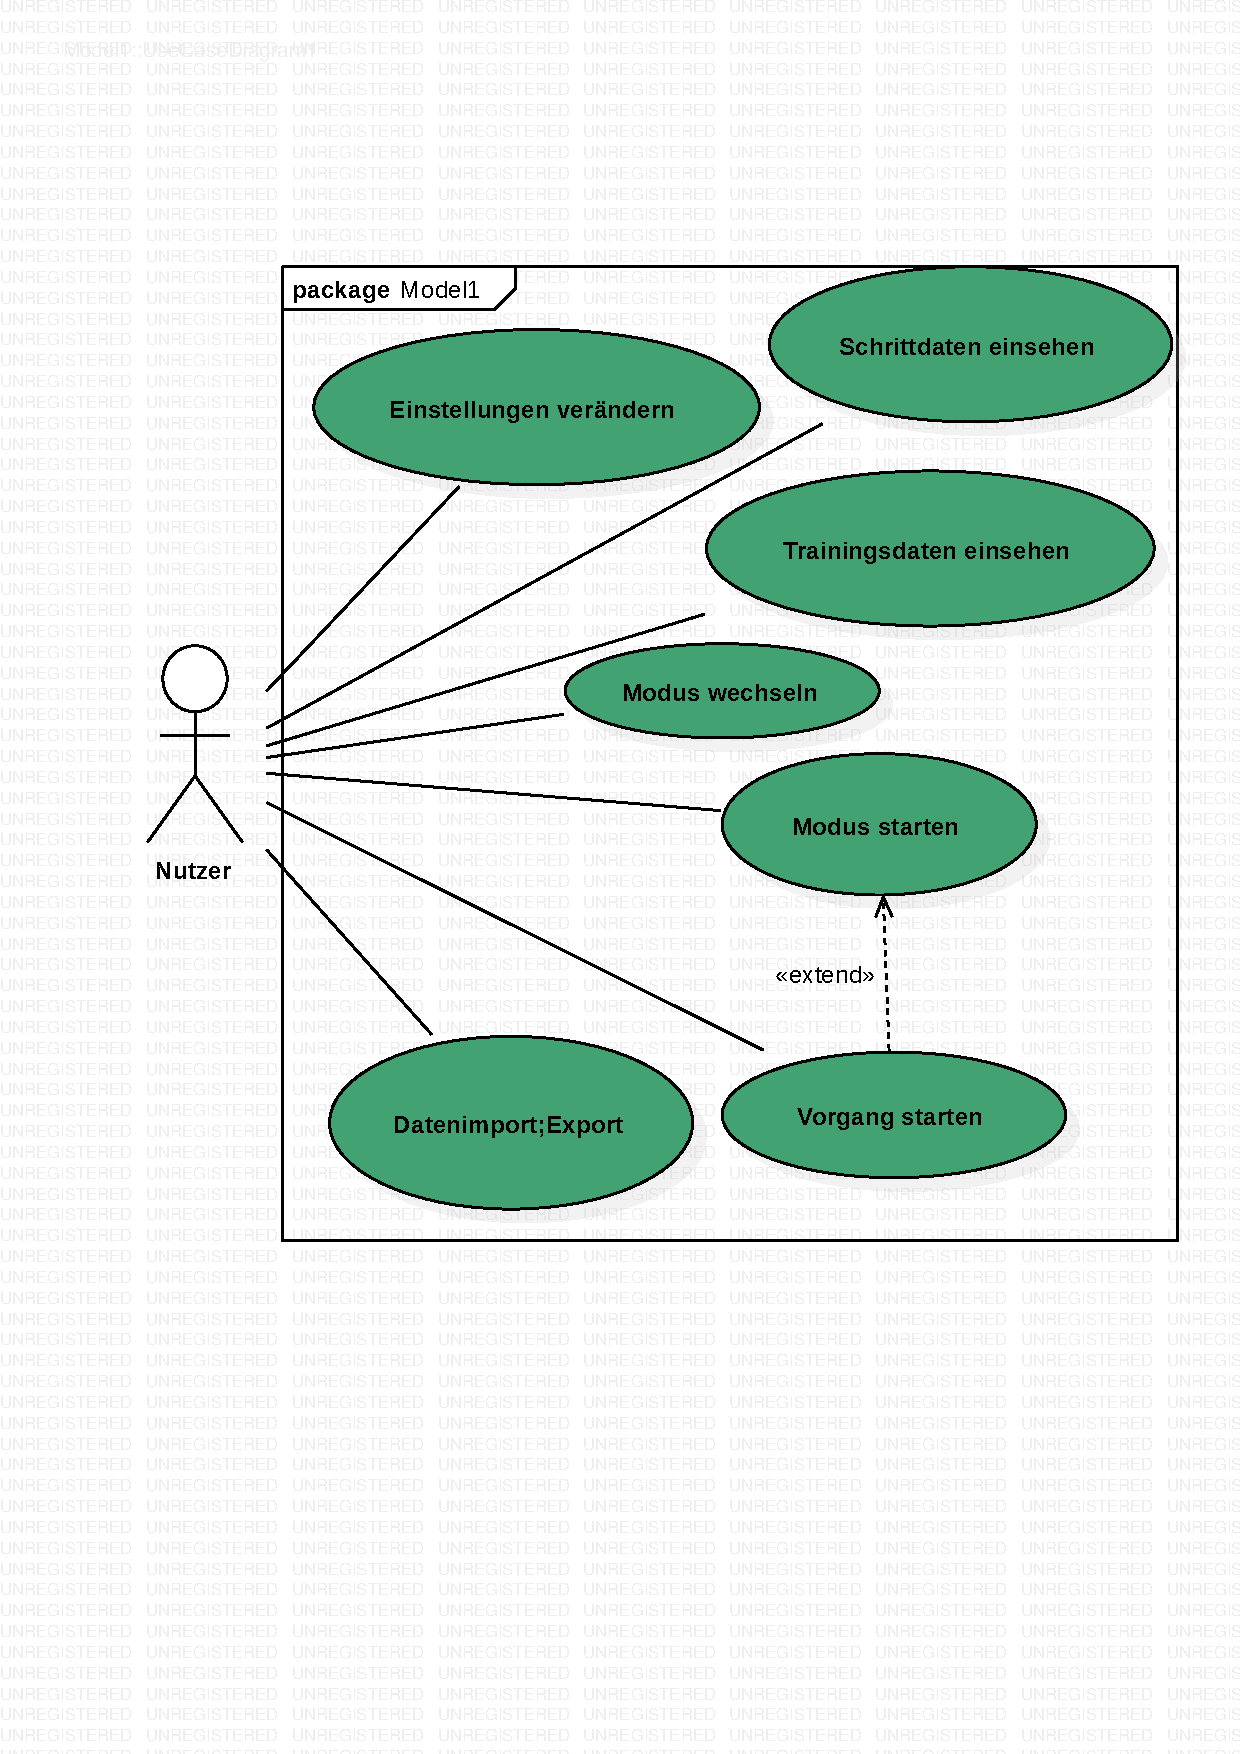
\includegraphics[width=0.8\textwidth]{Vorlaeufiges Use-Case Diagram.pdf} %%Textuelle Beschreibung wird noch ergänzt.
\end{center}
\section{Benutzeroberfläche}
%%TODO Benni auseinandersetzen
\section{Qualitätszielbestimmungen}
\begin{tabular}[t]{|c|c|c|c|c|c|}
  \hline
  \textbf{Kriterium} & \textbf{Sehr Wichtig} & \textbf{Wichtig} & \textbf{Weniger Wichtig} & \textbf{Unwichtig}\\
  \hline
  \hline
  Korrektheit & x & & &\\
  \hline
  Zuverlässigkeit & x & & &\\
  \hline
  Robustheit & x & & &\\
  \hline
  Effizienz & x & & &\\
  \hline
  Benutzerfreundlichkeit & x & & &\\
  \hline
  Vertrauenswürdigkeit & x & & &\\
  \hline

\end{tabular}

 %%!! Was ist hiermit? Stand noch in der Mail als Unterpunkt. https://www.sosy-lab.org/Teaching/2015-WS-SEP/samples/pflichtenheft.pdf Seite 13 sieht man so eine Tabelle, wie ist das gemeint?
 %%nächstes Treffen: ***kurzes*** Planungspoker mit Korrektheit, Zuverlässigkeit, Robustheit, Effizienz, Benutzerfreundlichkeit und Vertrauenswürdigkeit zwischen sehr wichtig, wichtig, weniger wichtig und unwichtig.
 %% code-standards??
\section{Globale Testfälle und Szenarien}
%%TODO David
  \subsection{Globale Testfälle}
  \subsubsection{Mussanforderungen}
  \paragraph{Laufmodus (/F100/)}
  \begin{enumerate}
    \item Das Smartphone wird per Bluetooth mit den Kopfhörern verbunden.
    \item Die App wird gestartet.
    \item Nach dem Startvorgang der App wird in den Modus \glqq Laufmodus\grqq{} gewechselt. %%Automatisch im Laufmodus?
    \item Die Kopfhörer werden korrekt am Ohr des Nutzers angebracht. %%Würde ich als ersten Schritt machen, da durch das Anbringen der Kopfhörer laufend angezeigt werden könnte
    \item Die App zeigt dem Nutzer den Status \glqq stehend\grqq{} an.
    \item Sobald der Nutzer anfängt zu gehen zeigt die App \glqq gehend\grqq{} an.
    \item Sobald der Nutzer wieder still steht ändert sich der Zustand wieder zurück zu \glqq stehend\grqq. 
  \end{enumerate}

  \subsubsection{Wunschanforderungen}
  %%vielleicht ohne absätze als Fließtext? -valle
  \paragraph{Start/Stop Musikmodus (/F210/)}
  \begin{itemize}
    \item[] Das Smartphone wird per Bluetooth mit den Kopfhörern verbunden.
    \item[] Der Nutzer spielt Musik mit der vorinstallierten Musik-App ab.
    \item[] Die App wird gestartet.
    \item[] Nach dem Startvorgang der App wird in den Modus \glqq Start/Stop Musikmodus\grqq{} gewechselt.
    \item[] Die Kopfhörer werden korrekt am Ohr des Nutzers angebracht.
    \item[] Der Nutzer beginnt zu gehen.
    \item[] Der Nutzer startet den gewählten Modus.
    \item[] Der Nutzer hört auf zu gehen.
    \item[] Die Musik wird pausiert.
    \item[] Der Nutzer geht weiter.
    \item[] Die Musik startet automatisch wieder.
  \end{itemize}
  
  \paragraph{Zählmodus (/F200/)}
  \begin{itemize}
    \item[] Das Smartphone wird per Bluetooth mit den Kopfhörern verbunden.
    \item[] Die App wird gestartet.
    \item[] Nach dem Startvorgang der App wird in den Modus \glqq Zählmodus\grqq{} gewechselt.
    \item[] Die Kopfhörer werden korrekt am Ohr des Nutzers angebracht.
    \item[] Der Nutzer wählt eine verfügbare Übung aus. 
    \item[] Der Nutzer startet den gewählten Modus.
    \item[] Der Nutzer führt die Übung X (natürliche Zahl) mal aus.
    \item[] Der Nutzer stoppt den laufenden Modus.
    \item[] Die App zeigt X an.
  \end{itemize}

  \paragraph{Livedaten (/F190/)}
  \begin{itemize}
    \item[] Das Smartphone wird per Bluetooth mit den Kopfhörern verbunden.
    \item[] Die App wird gestartet.
    \item[] Nach dem Startvorgang der App wird in den Modus \glqq Livedaten\grqq{} gewechselt.
    \item[] Die Kopfhörer werden korrekt am Ohr des Nutzers angebracht.
    \item[] Der Nutzer startet den gewählten Modus.
    \item[] Die App zeigt die korrekten Sensordaten 
  \end{itemize}

  \paragraph{Lauschen\&Agieren (/F220/)}
  \begin{itemize}
    \item[] Das Smartphone wird per Bluetooth mit den Kopfhörern verbunden.
    \item[] Die App wird gestartet.
    \item[] Nach dem Startvorgang der App wird in den Modus \glqq Lauschen\&Agieren\grqq{} gewechselt.
    \item[] Die Kopfhörer werden korrekt am Ohr des Nutzers angebracht.
    \item[] Der Nutzer stellt sich ein Training aus den verfügbaren Übungen zusammen (/F220/).
    \item[] Der Nutzer startet den gewählten Modus.
    \item[] Dem Nutzer wird per \Gls{TTS} die aktuelle Übung angesagt (/F230/).
    \item[] Der Nutzer führt die Übung aus.
    \item[] Die letzten beiden Schritte werden so lange wiederholt, bis alle ausgewählten Übungen erledigt sind.
    \item[] Der Modus wird automatisch beendet.
    \item[] Die App zeigt die benötigten Zeiten pro Übung an (/F240/).
  \end{itemize}

  \paragraph{Einstellungen (/F250/ bis /F285/)}

  \paragraph{Erstnutzung (/F290/)}

  \paragraph{Importieren/Exportieren (/F300/)}


  \subsection{Szenarien}
    \subsubsection{Bibliotheksnutzung}


\section{Entwicklungsumgebung}
Wir arbeiten an dem Projekt mit Visual Studio 2019, sodass alle eine einheitliche Entwicklungsumgebung verwenden.\\
Dabei kommt der .NET Standard 2.0 zum Einsatz, der C\# 7.2 verwendet. Wir arbeiten außerdem mit Xamarin Forms.\\
Zur Versionskontrolle und zur Projektübersicht wird Git verwendet, das Repository liegt öffentlich auf Github\footnote{\url{https://github.com/vlle1/earablesKIT}}.
\clearpage
\printglossaries
\stepcounter{section}
\end{document}
